% Figure from MATH 591 notes, section 8. Compile with the notes preamble.
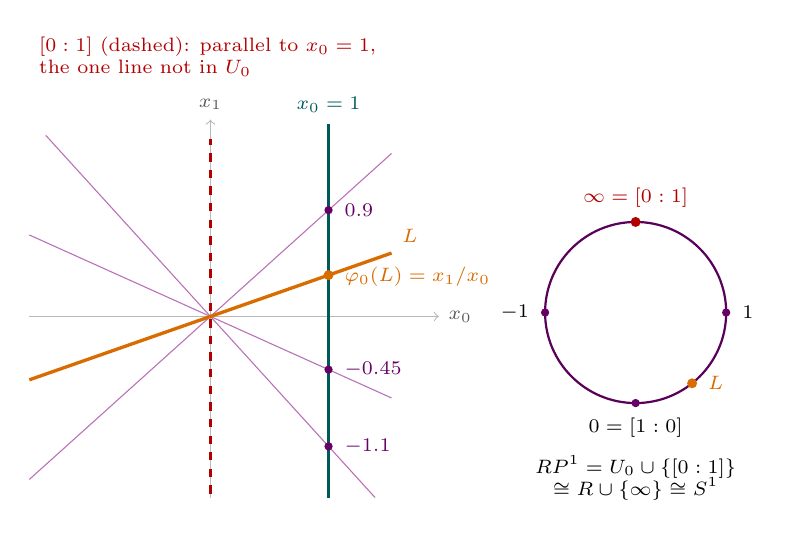
\begin{tikzpicture}
\draw[->, gray!55] (-2.3,0) -- (2.9,0) node[right, font=\scriptsize, text=gray!70!black] {$x_0$}; \draw[->, gray!55] (0,-2.3) -- (0,2.5) node[above, font=\scriptsize, text=gray!70!black] {$x_1$};
\draw[teal!70!black, very thick] (1.50,-2.3) -- (1.50,2.45) node[above, font=\scriptsize] {$x_0 = 1$};
\draw[violet!55] (-2.091,2.300) -- (2.091,-2.300);
\fill[violet!80!black] (1.500,-1.650) circle (1.5pt); \node[font=\scriptsize, anchor=west, text=violet!80!black] at (1.580,-1.650) {$-1.1$};
\draw[violet!55] (-2.300,1.035) -- (2.300,-1.035);
\fill[violet!80!black] (1.500,-0.675) circle (1.5pt); \node[font=\scriptsize, anchor=west, text=violet!80!black] at (1.580,-0.675) {$-0.45$};
\draw[violet!55] (-2.300,-2.070) -- (2.300,2.070);
\fill[violet!80!black] (1.500,1.350) circle (1.5pt); \node[font=\scriptsize, anchor=west, text=violet!80!black] at (1.580,1.350) {$0.9$};
\draw[orange!85!black, very thick] (-2.300,-0.805) -- (2.300,0.805) node[above right, font=\scriptsize] {$L$};
\fill[orange!85!black] (1.500,0.525) circle (1.8pt); \node[font=\scriptsize, anchor=west, text=orange!85!black] at (1.580,0.505) {$\varphi_0(L) = x_1/x_0$};
\draw[red!70!black, very thick, dashed] (0,-2.25) -- (0,2.25); \node[red!70!black, font=\scriptsize, align=left, anchor=west] at (-2.3,3.3) {$[0:1]$ (dashed): parallel to $x_0 = 1$,\\ the one line not in $U_0$};
\draw[thick, violet!70!black] (5.40,0.05) circle (1.15);
\fill[violet!80!black] (5.400,-1.100) circle (1.5pt); \node[font=\scriptsize, anchor=north] at (5.400,-1.160) {$0 = [1:0]$};
\fill[violet!80!black] (6.550,0.050) circle (1.5pt); \node[font=\scriptsize, anchor=west] at (6.630,0.050) {$1$};
\fill[violet!80!black] (4.250,0.050) circle (1.5pt); \node[font=\scriptsize, anchor=east] at (4.170,0.050) {$-1$};
\fill[orange!85!black] (6.117,-0.849) circle (1.8pt); \node[font=\scriptsize, anchor=west, text=orange!85!black] at (6.197,-0.849) {$L$};
\fill[red!70!black] (5.40,1.20) circle (1.8pt); \node[red!70!black, font=\scriptsize, anchor=south] at (5.40,1.26) {$\infty = [0:1]$};
\node[font=\scriptsize, align=center] at (5.40,-2.05) {$\mathbb{RP}^1 = U_0 \cup \{[0:1]\}$\\ $\cong \mathbb{R} \cup \{\infty\} \cong S^1$};
\end{tikzpicture}
